\documentclass[12pt,oneside]{article}
\usepackage{float}
\usepackage{amsfonts}
\usepackage{amsmath,amsthm,amssymb}
\usepackage{graphicx}
\usepackage[colorlinks=true]{hyperref}
\usepackage{cancel}
\usepackage[english]{babel}
\usepackage{blindtext}
\usepackage{media9}
\usepackage{color}
\usepackage{multicol}
\usepackage{units}
\usepackage[utf8]{inputenc}
\usepackage[T1]{fontenc}
\usepackage{longtable}

\setlength{\textheight}{9.5in}
\setlength{\textwidth}{7in}
\setlength{\topmargin}{-1in}
\setlength{\oddsidemargin}{-0.25in}
\setlength{\evensidemargin}{-0.5in}
\setlength{\parskip}{0.15in}
\setlength{\parindent}{0in}


\usepackage[usenames,dvipsnames]{xcolor}  %%%this package is required for latex code in svg graphics

\usepackage{titlesec}
\titlespacing*{\chapter}{0pt}{-50pt}{20pt}
\titleformat{\chapter}[display]{\normalfont\huge\bfseries}{\chaptertitlename\ \thechapter}{20pt}{\Huge}



%Various math operator macros
\DeclareMathOperator{\tr}{trace}
\DeclareMathOperator{\edm}{End}
\DeclareMathOperator{\Hom}{Hom}
\DeclareMathOperator{\im}{im}
\DeclareMathOperator{\ord}{ord}
\DeclareMathOperator{\rk}{rank}
\DeclareMathOperator{\card}{card}
\DeclareMathOperator{\len}{length}
\DeclareMathOperator{\supp}{supp}
\DeclareMathOperator{\rad}{rad}
\DeclareMathOperator{\spa}{span}
\DeclareMathOperator{\lcm}{lcm}

%Division symbols
\newcommand\dn{\!\nmid\!}
\newcommand\dv{\!\mid\!}

%Absolute values and norms
\newcommand{\abs}[1]{\lvert#1\rvert}
\newcommand{\norm}[1]{\lVert#1\rVert}

%Coloring the text
\newcommand{\red}{\textcolor{red}}
\newcommand{\green}{\textcolor{green}}
\newcommand{\blue}{\textcolor{blue}}
\newcommand{\yellow}{\textcolor{yellow}}
\newcommand{\brown}{\textcolor{brown}}
\newcommand{\pink}{\textcolor{pink}}
\newcommand{\magenta}{\textcolor{magenta}}
\newcommand{\purple}{\textcolor{purple}}
\newcommand{\orange}{\textcolor{orange}}

%Calligraphic symbols
\newcommand{\car}{{\cal R}}
\newcommand{\cm}{{\cal M}}
\newcommand{\ca}{{\cal A}}
\newcommand{\cl}{{\cal L}}
\newcommand{\ci}{{\cal I}}
\newcommand{\cj}{{\cal J}}
\newcommand{\ck}{{\cal K}}
\newcommand{\cn}{{\cal N}}
\newcommand{\cq}{{\cal Q}}
\newcommand{\ce}{{\cal E}}
\newcommand{\cp}{{\cal P}}
\newcommand{\cu}{{\cal U}}
\newcommand{\cf}{{\cal F}}
\newcommand{\cc}{{\cal C}}
\newcommand{\ct}{{\cal T}}

%Math blackboard bold symbols
\newcommand{\mba}{\mathbb{A}}
\newcommand{\mbr}{\mathbb{R}}
\newcommand{\mbz}{\mathbb{Z}}
\newcommand{\mbq}{\mathbb{Q}}
\newcommand{\mbf}{\mathbb{F}}
\newcommand{\mbn}{\mathbb{N}}
\newcommand{\mbc}{\mathbb{C}}
\newcommand{\mbp}{\mathbb{P}}
\newcommand{\mbe}{\mathbb{E}}
\newcommand{\zns}{\mathbb{Z}_n^\star}
\newcommand{\zps}{\mathbb{Z}_p^\star}

%Making matrices
\newcommand{\bbm}{\begin{bmatrix}}
\newcommand{\ebm}{\end{bmatrix}}
\newcommand{\bpm}{\begin{pmatrix}}
\newcommand{\epm}{\end{pmatrix}}

%Polynomial ring shortcuts
\newcommand{\kx}{K[X]}
\newcommand{\fx}{F[X]}
\newcommand{\rx}{R[X]}
\newcommand{\ax}{A[X]}
\newcommand{\bx}{B[X]}
\newcommand{\krx}{K(X)}
\newcommand{\frx}{F(X)}
\newcommand{\lx}{L[X]}
\newcommand{\qrx}{\mathbb{Q}(X)}
\newcommand{\zx}{\mathbb{Z}[X]}
\newcommand{\rex}{\mathbb{R}[X]}
\newcommand{\cx}{\mathbb{C}[X]}
\newcommand{\qx}{\mathbb{Q}[X]}
\newcommand{\zpx}{\mathbb{Z}_p[X]}

%Greek shortcuts
\newcommand{\ag}{\alpha}
\newcommand{\al}{\alpha}
\newcommand{\vf}{\varphi}
\newcommand{\ve}{\varepsilon}

%Peripheral symbols
\newcommand{\ar}{\rightarrow}
\newcommand{\iiff}{\Longleftrightarrow}
\newcommand{\ol}{\overline}
\newcommand{\la}{\langle}
\newcommand{\ra}{\rangle}
\newcommand{\gi}{\mbz[i]}

%Makes dispalystyle
\newcommand{\dss}{\displaystyle}

%Sets up a unnumbered subsubsection 
\newcommand{\sss}{\subsubsection*}

%makes the mod notation
\newcommand\md{\!\!\!\mod}

%Puts the marks in the margins
\newcommand{\rmp}{\reversemarginpar\marginpar}

% \highlight[<colour>]{<stuff>}
\newcommand{\highlight}[2][yellow]{\mathchoice%
  {\colorbox{#1}{$\displaystyle#2$}}%
  {\colorbox{#1}{$\textstyle#2$}}%
  {\colorbox{#1}{$\scriptstyle#2$}}%
  {\colorbox{#1}{$\scriptscriptstyle#2$}}}%

\usepackage{lipsum}% http://ctan.org/pkg/lipsum
\usepackage{eso-pic}% http://ctan.org/pkg/eso-pic
\usepackage{graphicx}% http://ctan.org/pkg/graphicx


\newcommand*\circled[1]{\tikz[baseline=(char.base)]{
            \node[shape=circle,draw,inner sep=2pt] (char) {#1};}}


\DeclareMathSizes{12}{15}{14}{14}

\newcommand{\uph}[1]{\underline{#1}}
\newcommand{\NMarks}[1]{{\textcolor{magenta}{[#1 marks]}}}
\newcommand{\Score}[1]{\hfill{\LARGE \textcolor{magenta}{Score: }}{\Huge \textcolor{magenta}{$\displaystyle \frac{}{#1}$\\}}}

\usepackage[most]{tcolorbox}

\newcommand{\partone}{
    \begin{tcolorbox}[breakable, enhanced, colframe=blue!25,
    colback=white!10,
    coltitle=blue!20!black,  
    title= {\bf Task 1: Basic Tuning Fork Frequencies.}] 
    For your first task, you are to measure the frequencies of the set of tuning forks provided in class. Using the virtual oscilloscope at \url{https://academo.org/demos/virtual-oscilloscope/}, you will record a clear sound wave for each of the tuning forks. Take a screen-shot of the image and approximate the wavelength from the graph. Using the formula $f=\tfrac{1}{\lambda}$, where $\lambda$ is the wavelength, approximate the frequency of each tuning fork (8 separate computations) \underline{and} measure the percent error in comparison with the frequency written on the respective tuning forks.
    \end{tcolorbox}
}

\newcommand{\parttwo}{
    \newpage
    \begin{tcolorbox}[breakable, enhanced, colframe=blue!25,
        colback=white!10,
        coltitle=blue!20!black,  
        title= {\bf Task 2: Combining Sinusoidals.}] 
        For your second task, you will be playing two tuning forks at once. Ideally, these should be played at amplitudes (loudness) that are as similar as possible. Using the formula:
        $$\sin\left(2\pi f_1 t\right) + \sin\left(2\pi f_2 t\right) = 2\cos\left(2\pi\cdot \dss\frac{f_1-f_2}{2}\cdot t\right)\sin\left(2\pi\cdot \dss\frac{f_1+f_2}{2}\cdot t\right)$$
        where $f_1$ and $f_2$ are the frequencies, you will be computing the theoretical function formed by playing two tuning forks simultaneously and comparing this with your experimental results. To do so, you will need to take screen-shots of the resultant sound waves, making sure you capture the fluctuations in amplitude as well. Then, using a dynamic geometry software such as GeoGebra or Desmos, you will graph the theoretical function you obtained from the identity above and then layer over it the screen-shot you took to see how well they match. This will require you to make the layered image opaque (increase its transparency) and will require some horizontal and vertical scaling of the image to match the function. Once you have successfully layered these together, take a screen-shot of the two waves \underline{and} comment on how well matched your results are to the expected values, including discussing the possible sources of error in your computations. You will need to perform this task on three different combinations of tuning forks (ex. A \& B, B \& F, D \& G). Clearly indicate which grouping you are using in your submission.\\
        \end{tcolorbox}
}

\newcommand{\partthree}{
    \newpage
    \begin{tcolorbox}[breakable, enhanced, colframe=blue!25,
        colback=white!10,
        coltitle=blue!20!black,  
        title= {\bf Task 3: Drop a Beat!}] 
        For this task, you will creating \underline{\bf three different beats} using the beat generator at Academo.org, which you can find at \url{https://academo.org/demos/wave-interference-beat-frequency/}. To do so, you will need to choose two frequencies that are close together, turn the sound on, and take a screen-shot of your set-up \underline{as well as} an audio recording of the beat created. You will then need to either include the audio directly into your assignment or include a link to a Google Drive recording to hear the beat. The screen-shot taken must clearly show the frequencies of the initial waves and the resulting beats (3-4 envelopes, as shown in class). 
        \end{tcolorbox}
}

\providecommand{\tightlist}{%
  \setlength{\itemsep}{0pt}\setlength{\parskip}{0pt}}


\begin{document}

\noindent
\magenta{\Large{\bf Enriched 11 IB Mathematics A\&A HL Y1 \hfill {2020-21}}\\
\underline{\Large{\bf The Music of Trigonometry}}\\}

\magenta{\large{\bf M. Hoteit}\\\\
\large{\underline{Due Date:}\quad  Thursday, Feb 18 2021 10 PM}}\par
\vspace{0.015in}\hrulefill\ \\
\begin{minipage}{\textwidth}
    \centering
    \vspace{0.15in}
    \Large{\bf The Music of the Sines}\par
    \vspace{0.15in}
\end{minipage}
\large{First Group Member: Edouard Des Parois Perrault}
\par
\large{Second Group Member: Juliette Kwan}
\par
\large{Third Group Member: Justin Ho}
\\

\normalsize

%%%%%%REPLACE ALL THE RED TEXT BELOW WITH YOUR ANSWERS%%%%%%

\textbf{Reference Declaration}

Complete the Reference Declaration section below in order for your assignment to be graded.

If you used any references beyond the course text and lectures (such as other texts, discussions with classmates or online resources), indicate this information in the space below.  If you did not use any aids, state this in the space provided. 

Note: Your submitted work must be \textbf{your original work}. 

\underline{Declared References:} \\

\begin{enumerate}
    \item We spoke to Arthur Huang and Tram-Anh Ngo's team for clarifications on
our results
    \item We spoke to Justin Huang's team for clarifications on our results
\end{enumerate}

\newpage

\partone

\textbf{Please Note:} For each of the graphs in this section, the scale
was kept consistent; each division is one millisecond.

\begin{enumerate}
\item \underline{\bf C Tuning Fork - 512 Hz:}

\color{red}

\begin{figure}[H]

{\centering 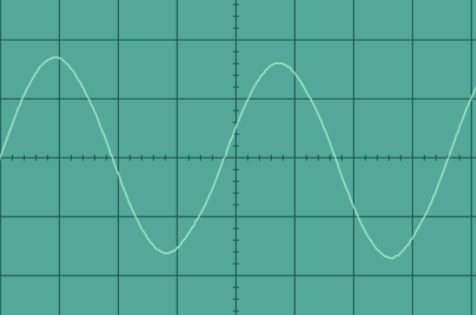
\includegraphics[width=15cm,]{./images/c4} 

}

\caption{C4 Fork Graph}\label{fig:c4}
\end{figure}

\begin{eqnarray}
\text{freq} & = & 0.2 \cdot 19.5 \\
            & = & 3.9 \\
            & = & \frac{39}{1000} \\
            & = & 0.0039 \\
            & = & \frac{1}{0.0039} \\
            & = & 256.41
\end{eqnarray}

See Figure \ref{fig:c4} for image.

\textbf{Frequency:} 256.41 Hz

\par

\textbf{Expected Frequency:} 256 Hz

\par

\textbf{Percent Error: } 0.2\%

\color{black}

\item \underline{\bf B Tuning Fork - 480 Hz:}
\color{red}

\begin{figure}[H]

{\centering 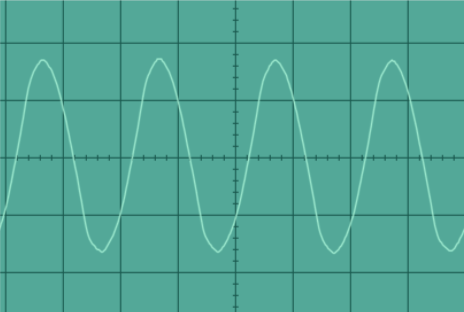
\includegraphics[width=15cm,]{./images/b4} 

}

\caption{B Tuning Fork Graph}\label{fig:b4}
\end{figure}

\begin{eqnarray}
  \text{freq} & = & 0.2 \cdot 10 \\
              & = & 2 \\
              & = & \frac{2}{1000} \\
              & = & 0.002 \\
              & = & \frac{1}{002} \\
              & = & 500
\end{eqnarray}

See Figure \ref{fig:b4} for image.

\textbf{Frequency:} 500 Hz

\par

\textbf{Expected Frequency:} 480 Hz

\par

\textbf{Percent Error: } 4\%

\color{black}

\item \underline{\bf A Tuning Fork - 426.6 Hz:}
\color{red}

\begin{figure}[H]

{\centering 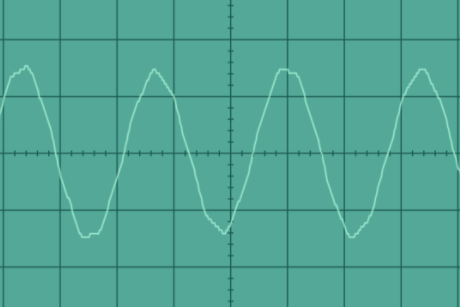
\includegraphics[width=15cm,]{./images/a4} 

}

\caption{A Tuning Fork Graph}\label{fig:a4}
\end{figure}

\begin{eqnarray}
  \text{freq} & = & 0.2 \cdot 12 \\
              & = & 2.4 \\
              & = & \frac{2.4}{1000} \\
              & = & 0.0024 \\
              & = & \frac{1}{0024} \\
              & = & 416.67
\end{eqnarray}

See Figure \ref{fig:a4} for image.

\textbf{Frequency:} 416.67 Hz

\par

\textbf{Expected Frequency:} 426.6 Hz

\par

\textbf{Percent Error: } 2.33\%

\color{black}

\item \underline{\bf G Tuning Fork - 384 Hz:}
\color{red}

\begin{figure}[H]

{\centering 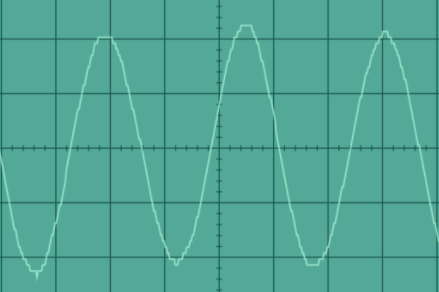
\includegraphics[width=15cm,]{./images/g4} 

}

\caption{G4 Tuning Fork Graph}\label{fig:g4}
\end{figure}

\begin{eqnarray}
  \text{freq} & = & 0.2 \cdot 12.5 \\
              & = & 2.5 \\
              & = & \frac{2.5}{1000} \\
              & = & 0.0025 \\
              & = & \frac{1}{0.0025} \\
              & = & 400
\end{eqnarray}

See Figure \ref{fig:g4} for image.

\textbf{Frequency:} 400 Hz

\par

\textbf{Expected Frequency:} 384 Hz

\par

\textbf{Percent Error: } 4\%

\color{black}
\item \underline{\bf F Tuning Fork - 341.3 Hz:}
\color{red}

\begin{figure}[H]

{\centering 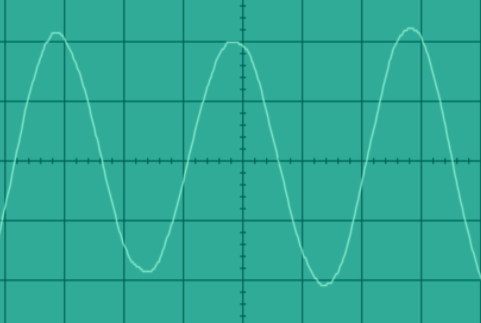
\includegraphics[width=15cm,]{./images/f4} 

}

\caption{F Tuning Fork Graph}\label{fig:f4}
\end{figure}

\begin{eqnarray}
  \text{freq} & = & 0.2 \cdot 15 \\
              & = & 3 \\
              & = & \frac{3}{1000} \\
              & = & 0.003 \\
              & = & \frac{1}{0.003} \\
              & = & 333.33
\end{eqnarray}

See Figure \ref{fig:f4} for image.

\textbf{Frequency:} 333.33 Hz

\par

\textbf{Expected Frequency:} 341.3 Hz

\par

\textbf{Percent Error: } 2\%

\color{black}
\item \underline{\bf E Tuning Fork - 320 Hz:}
\color{red}

\begin{figure}[H]

{\centering 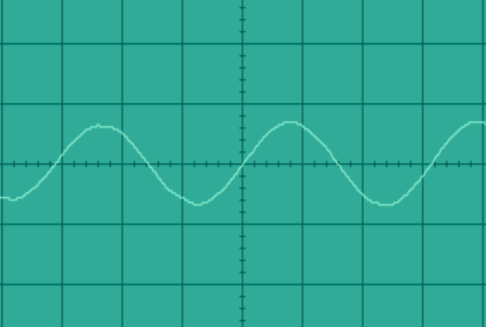
\includegraphics[width=15cm,]{./images/e4} 

}

\caption{E Tuning Fork Graph}\label{fig:e4}
\end{figure}

\begin{eqnarray}
  \text{freq} & = & 0.2 \cdot 16 \\
              & = & 3.2 \\
              & = & \frac{3.2}{1000} \\
              & = & 0.0032 \\
              & = & \frac{1}{0.0032} \\
              & = & 312.5
\end{eqnarray}

See Figure \ref{fig:e4} for image.

\textbf{Frequency:} 312.5 Hz

\par

\textbf{Expected Frequency:} 320 Hz

\par

\textbf{Percent Error: } 2\%

\color{black}
\item \underline{\bf D Tuning Fork - 288 Hz:}
\color{red}

\begin{figure}[H]

{\centering 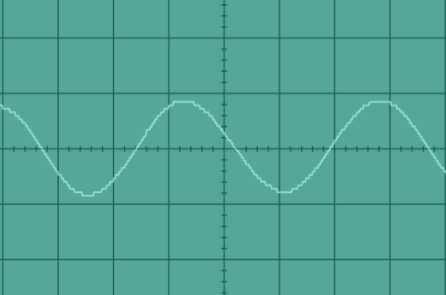
\includegraphics[width=15cm,]{./images/d4} 

}

\caption{D Tuning Fork Graph}\label{fig:d4}
\end{figure}

\begin{eqnarray}
  \text{freq} & = & 0.2 \cdot 17.5 \\
              & = & 3.5 \\
              & = & \frac{3.5}{1000} \\
              & = & 0.0035 \\
              & = & \frac{1}{0.0035} \\
              & = & 285.71
\end{eqnarray}

See Figure \ref{fig:d4} for image.

\textbf{Frequency:} 285.71 Hz

\par

\textbf{Expected Frequency:} 288 Hz

\par

\textbf{Percent Error: } 1\%

\color{black}
\item \underline{\bf C Tuning Fork - 256 Hz:}
\color{red}

\begin{figure}[H]

{\centering 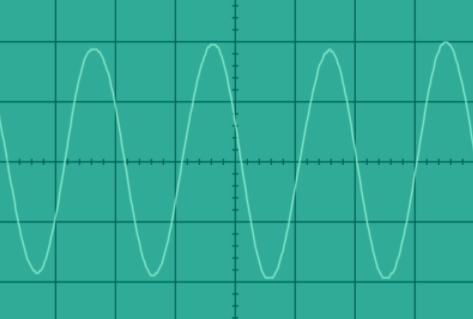
\includegraphics[width=15cm,]{./images/c5} 

}

\caption{C5 Tuning Fork Graph}\label{fig:c5}
\end{figure}

\begin{eqnarray}
  \text{freq} & = & 0.2 \cdot 9.5 \\
              & = & 1.9 \\
              & = & \frac{1.9}{1000} \\
              & = & 0.0019 \\
              & = & \frac{1}{0.0019} \\
              & = & 526.32
\end{eqnarray}

See Figure \ref{fig:c5} for image.

\textbf{Frequency:} 526.32 Hz

\par

\textbf{Expected Frequency:} 512 Hz

\par

\textbf{Percent Error: } 3\%

\end{enumerate}

\parttwo

\textbf{Note:} In the interest of keeping this report succinct, let the
basic form of the function \(C(x)\) be
\(2\cos\left(2\pi\cdot\frac{f_1 - f_2}{2}\cdot x\right)\sin\left(2\pi\cdot\frac{f_1 + f_2}{2}\cdot x\right)\),
with \(f_1\) and \(f_2\) being the frequencies of the two different
notes being summed up.

\begin{enumerate}

\item \underline{\bf First combination (state clearly which notes and their frequencies):}
\color{red}
%%%%include screen-shots and calculations here using different colour.

\textbf{First Note:} F4 (341.1 Hz)

\par

\textbf{Second Note:} B4 (480 Hz)

\begin{figure}[H]

{\centering 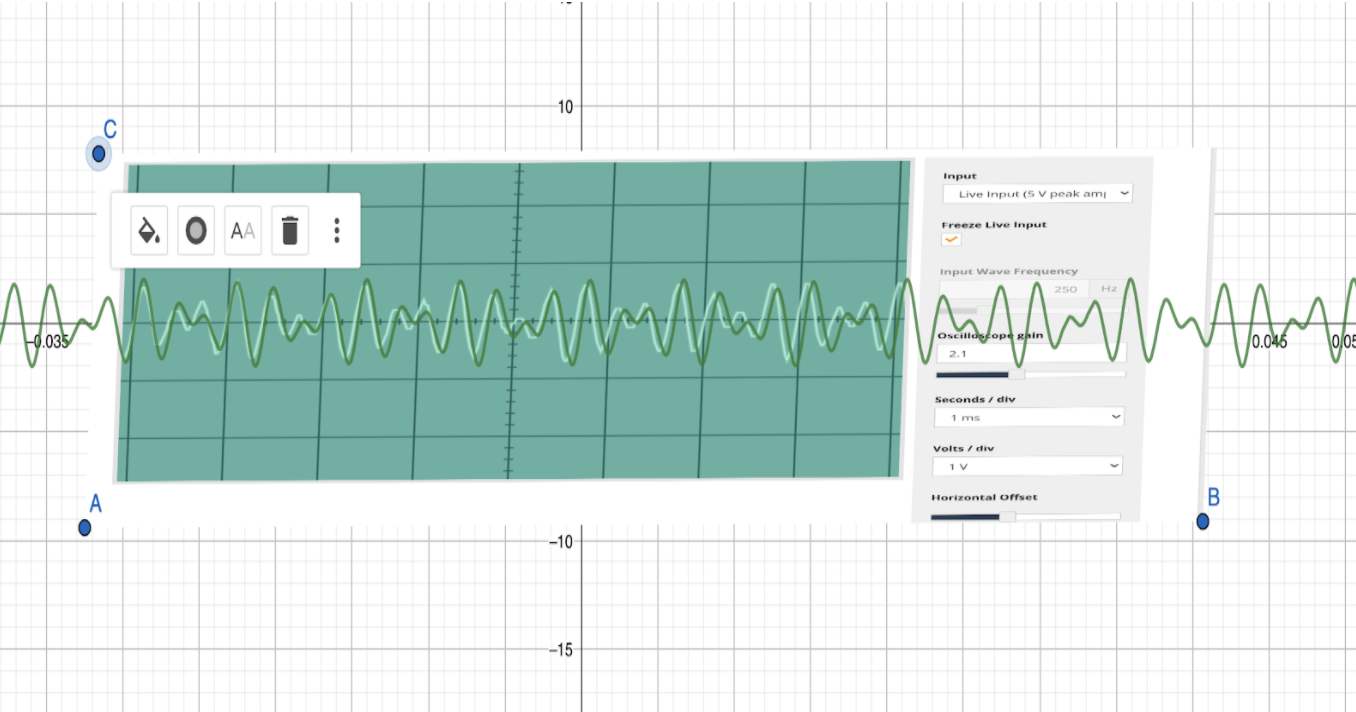
\includegraphics[width=15cm,]{./images/fandb} 

}

\caption{First Combination}\label{fig:combo-1}
\end{figure}

\textbf{Calculations:} \begin{eqnarray}
  A(x) & = & \sin (2\pi\cdot 341.1\cdot x) \\
  B(x) & = & \sin (2\pi\cdot 480 \cdot x) \\
  C(x) & = & A(x) + B(x) \\
       & = & 2\cos\left(2\pi\cdot\frac{480 - 341.1}{2}\cdot x\right)\sin\left(2\pi\cdot\frac{480 + 341.1}{2}\cdot x\right) \\
       & = & 2\cos\left(2\pi\cdot 69.45\cdot x\right)\sin\left(2\pi\cdot 410.55\cdot x\right)
\end{eqnarray}

\color{black}
\item \underline{\bf Second combination (state clearly which notes and their frequencies):}
%%%%include screen-shots and calculations here using different colour.
\color{red}

\textbf{First Note:} F4 (341.1 Hz)

\par

\textbf{Second Note:} G4 (384 Hz)

\begin{figure}[H]

{\centering 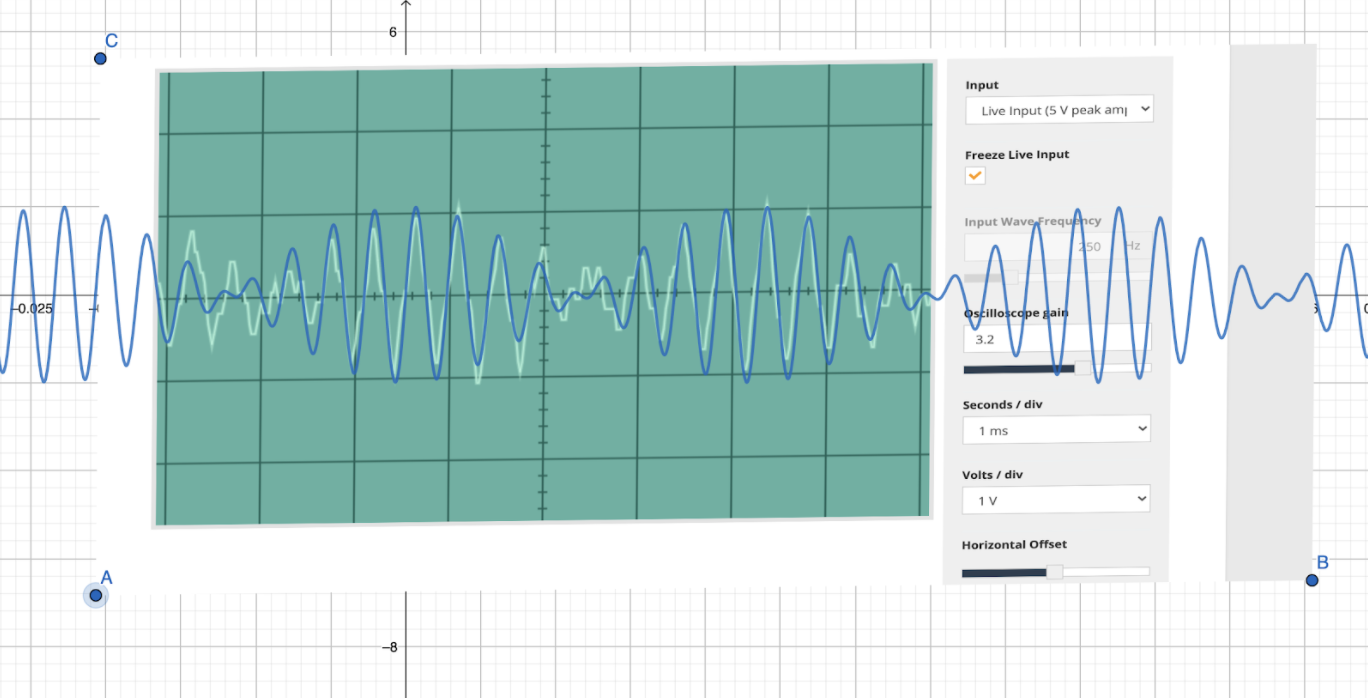
\includegraphics[width=15cm,]{./images/fandg} 

}

\caption{Second Beat}\label{fig:combo-2}
\end{figure}

\textbf{Calculations:}

\begin{eqnarray}
  A(x) & = & \sin (2\pi\cdot 341.1 \cdot x) \\
  B(x) & = & \sin (2\pi\cdot 384\cdot x) \\
  C(x) & = & A(x) + B(x) \\
       & = & 2\cos\left(2\pi\cdot\frac{384-341.1}{2}\cdot x\right)\sin\left(2\pi\cdot\frac{384-341.1}{2}\cdot x\right) \\ 
       & = & 2\cos\left(2\pi\cdot 21.45\cdot x\right)\sin\left(2\pi\cdot 362.9\cdot x\right)
\end{eqnarray}

\color{black}
\item \underline{\bf Third combination (state clearly which notes and their frequencies):}
%%%%include screen-shots and calculations here using different colour.
\color{red}

\textbf{First Note:} C5 (512 Hz)

\par

\textbf{Second Note:} G4 (384 Hz)

\begin{figure}[H]

{\centering 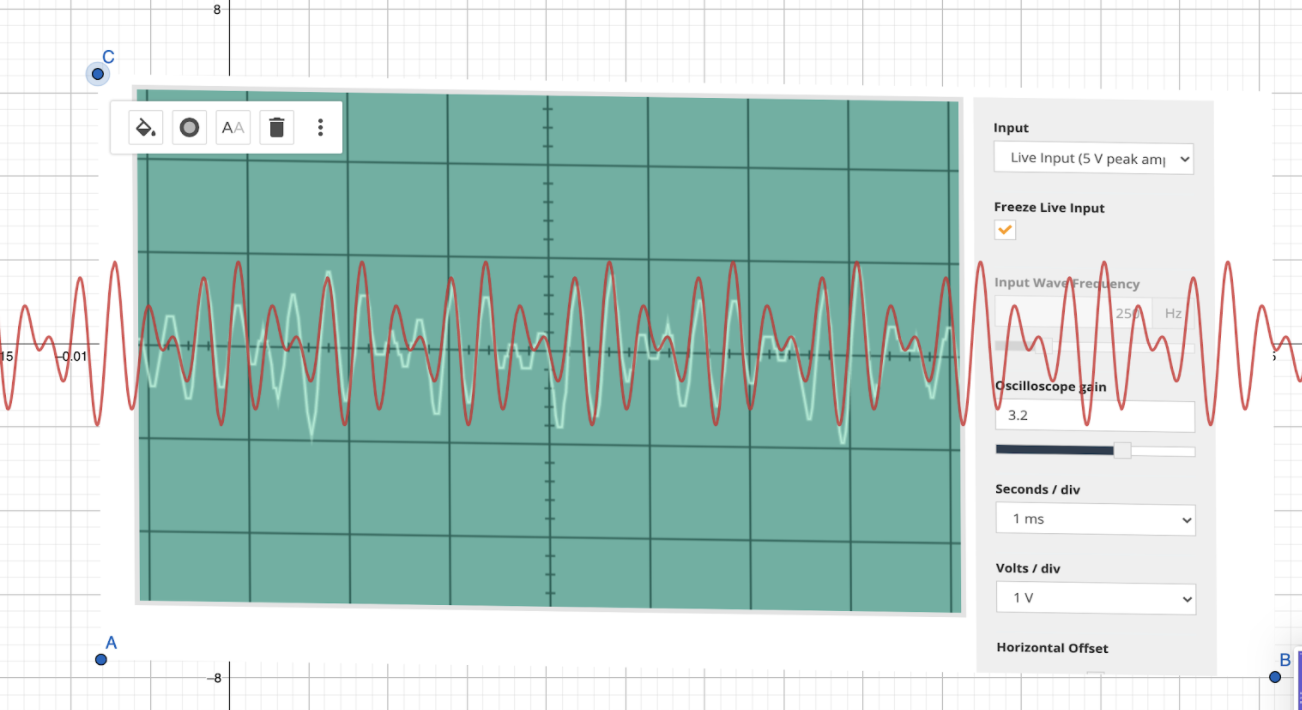
\includegraphics[width=15cm,]{./images/candg} 

}

\caption{Third Beat}\label{fig:combo-3}
\end{figure}

\textbf{Calculations:}

\begin{eqnarray}
  A(x) & = & \sin (2\pi\cdot 512 \cdot x) \\
  B(x) & = & \sin (2\pi\cdot 384\cdot x) \\
  C(x) & = & A(x) + B(x) \\
       & = & 2\cos\left(2\pi\frac{512-384}{2}\cdot x\right)\sin\left(2\pi\cdot\frac{512+384}{2}\cdot x\right) \\ 
       & = & 2\cos\left(2\pi\cdot64\cdot x\right)\sin\left(2\pi\cdot 448\cdot x\right)
\end{eqnarray}

\color{black}
\end{enumerate}
\color{red}

\textbf{Comments:} As per the instructions, comments should be made for
the results of this experiment, though we were unsure whether a separate
set of comments should be produced for each computation. Given that the
computations were rather repetitive, we have made the decision to only
include one set of comments for all trials at the end of this section.

\par

We have identified several sources of error, which we define in the
below list. We strongly believe that these sources of error are the
reasons why the composite waves we obtained were not exactly identical
to those produced by our graphing software. Indeed, in all cases, the
waves were close, though they were far from identical (see Figures
\ref{fig:combo-1}, \ref{fig:combo-2}, and \ref{fig:combo-3}).

\begin{enumerate}
\def\labelenumi{\arabic{enumi}.}
\tightlist
\item
  The imprecision of the tuning forks
\item
  The imprecision of the computer's microphone
\item
  The imprecision of the oscilloscope
\item
  Constructive interference due to the surrounding environment
\end{enumerate}

Further elaboration on each of these sources of error can be found
below.

\hypertarget{the-imprecision-of-the-tuning-forks}{%
\subsection*{The imprecision of the tuning
forks}\label{the-imprecision-of-the-tuning-forks}}
\addcontentsline{toc}{subsection}{The imprecision of the tuning forks}

We suspect it does not come as much of a surprise that the tuning forks
employed in this experiment were not very precise. Take the note F4, for
instance. \href{https://pages.mtu.edu/~suits/notefreqs.html}{A quick
google search} reveals that the accepted frequency of F4 is 349.23 Hz.
That said, the frequency inscribed on the F4 tuning fork was 341.1. This
is a percent error of 2.33\% right off the bat.

\par

In addition, some of the tuning forks were strangely identical, which
suggests that the the value was written on the each of the forks was
produced without any tests having been conducted to support it.

\par

We would like to share a quick test that can be conducted in order to
support this argument; take a tuning fork in a quiet environment and
make it vibrate. Consult an oscilloscope and take note of the frequency.
Then, use an electronic device capable of producing a pure sine wave
(i.e.~a phone) and play the same note into the oscilloscope in order to
record its wave. You will notice that the frequencies are different.
Even in a perfectly quiet room, the fork is unable to produce a pure
sine wave.

\par

Finally, in hindsight, the fact that the forks were repeatedly banged
against the wall probably did not aid their precision. By the end of the
experiment, many of them no longer had perfect edges. Although we
recognize our lack of expertise in the domain, we suspect that dents in
the forks must have introduced some sort of imprecision.

\par

\hypertarget{the-imprecision-of-the-computers-microphone}{%
\subsection*{The Imprecision of the Computer's
Microphone}\label{the-imprecision-of-the-computers-microphone}}
\addcontentsline{toc}{subsection}{The Imprecision of the Computer's
Microphone}

The mac we used was an A1708. Now, it is very difficult to obtain
technical specifications about it's microphone, apart from the fact that
it has one (thank you so much Apple), but
\href{https://www.macworld.com/article/2367142/understanding-the-limitations-of-a-macs-microphone.html}{a
quick Google search} reveals that it is far from being adequate to
recording anything above the quality of a FaceTime call. In other words,
the Mac microphone is great for speaking with a friend, but for
high-precision experiments, it is so subpar that Apple has decided not
to even post its specifications. In light of this, we suspect that it
may have been unable to faithfully record the waves we created.

\hypertarget{the-imprecision-of-the-osilloscope}{%
\subsection*{The Imprecision of the
Osilloscope}\label{the-imprecision-of-the-osilloscope}}
\addcontentsline{toc}{subsection}{The Imprecision of the Osilloscope}

Although the oscilloscope app we used had undeniable potential as an
educational tool, its quality was extremely questionable. For instance,
when we were calculating the wavelength, we counted the divisions and
approximated. Because each tick on the graph was 0.2 ms, the precision
of the oscilloscope itself was about \(\pm 0.1\)ms, and this does not
include the imprecision of the microphone, which may have been much
lower. The wavelength of middle C (C4) is about 3.9 milliseconds (in
theory), so the percent of the oscilloscope alone is about 3\%.
Moreover, changing the parameters of the oscilloscope seemed to produce
illogical results (though this may also have been due to the surrounding
environment), which suggests that there was perhaps a bug in the
underlying javascript code of the application.

\hypertarget{the-constructive-interference-due-to-the-surrounding-environment}{%
\subsection*{The Constructive interference due to the Surrounding
Environment}\label{the-constructive-interference-due-to-the-surrounding-environment}}
\addcontentsline{toc}{subsection}{The Constructive interference due to
the Surrounding Environment}

The room we conducted our tests in was far from silent despite it being
a library; we conducted our tests amid a symphony of chatter, of banging
tuning forks, and of shuffling students This undoubtedly produced some
interferance, which changed our results. We suspect that this was the
factor that contributed the most to the descrepancy between the
theoretical wave and the actual wave we obtained. A simple experiment
reveals this imprecision; measure the sine wave of the tuning fork in a
quiet room, and it takes two seconds and only one try to get an
acceptable wave (the precision of the forks themselves, however, is
another story). Do the same in a noisy room, and it can take several
tries to obtain the same results. Ambient noise has a significant part
to play when it comes to precision.

\color{black}

\partthree

\begin{enumerate}

\item \underline{\bf First beat:}
\color{red}

\begin{figure}[H]

{\centering 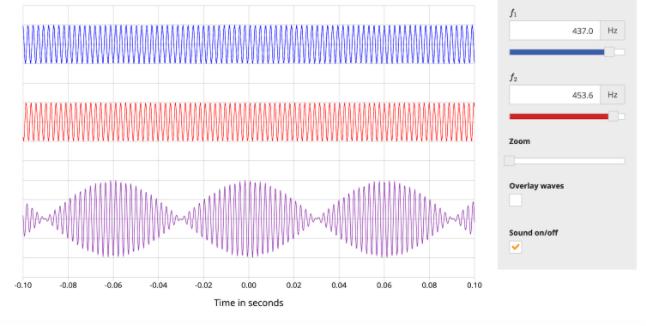
\includegraphics[width=15cm,]{./images/beat1} 

}

\caption{Graph of the First Beat}\label{fig:beat1}
\end{figure}

\textbf{Frequency 1:} 437 Hz

\par

\textbf{Frequency 2:} 453.6 Hz

\par

Click
\href{https://drive.google.com/file/d/1oXFQMKwtDi49notKpu_14QgbBMQKakrs/view?usp=sharing}{here}
to listen to the recording

\color{black}
\item \underline{\bf Second beat:}
\color{red}

\begin{figure}[H]

{\centering 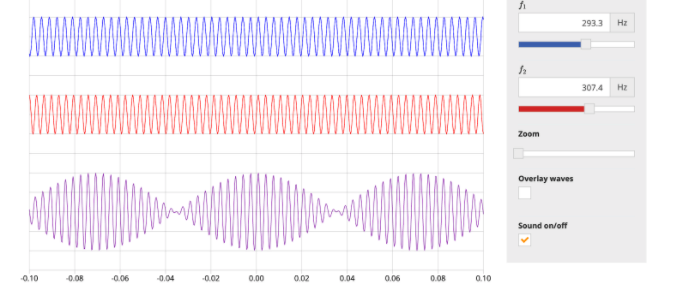
\includegraphics[width=15cm,]{./images/beat2} 

}

\caption{Graph of the Second Beat}\label{fig:beat2}
\end{figure}

\textbf{Frequency 1:} 293.3 Hz

\par

\textbf{Frequency 2:} 307.4 Hz

\par

Click
\href{https://drive.google.com/file/d/1oeeTuEsuQm12f_mGFPHBa7d3HnDYG668/view?usp=sharing}{here}
to listen to the recording

\color{black}
\item \underline{\bf Third beat:}
\color{red}

\begin{figure}[H]

{\centering 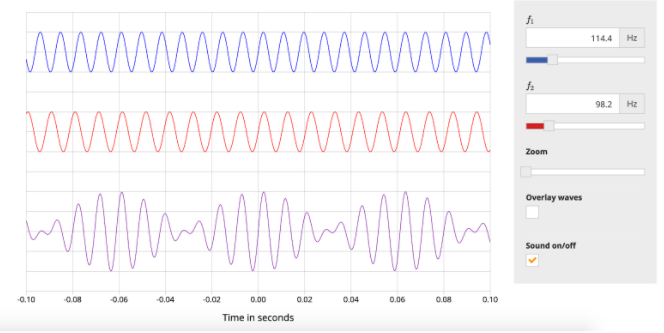
\includegraphics[width=15cm,]{./images/beat3} 

}

\caption{Graph of the Third Beat}\label{fig:beat3}
\end{figure}

\textbf{Frequency 1:} 114.4 Hz

\par

\textbf{Frequency 2:} 98.2 Hz

\par

Click
\href{https://drive.google.com/file/d/1HDnGARGU-zLe6rnKFT0szBtuhRpNQbNN/view?usp=sharing}{here}
to listen to the recording

\color{black}
\end{enumerate}

\end{document}